\documentclass{article}


\usepackage{graphicx}
\usepackage{hyperref}
\usepackage[utf8]{inputenc}
\usepackage[francais]{babel}


\title{De Révolution à Evolution \\ Création d'un jeu vidéo sur les thèmes de l'écologie et de la transition énergétique}
\date{16-02-2018}
\author{Niels Lachat \\ Mentor : Patrick Rickli}

\begin{document}
        \pagenumbering{gobble}
        \maketitle
        \newpage
        \pagenumbering{arabic}

        \tableofcontents
        \newpage

        \section{Introduction}
        Le but de ce travail de maturité était de créer un jeu vidéo abordant les thématiques de l'environnement et de la transition énergétique. Le genre du jeu de gestion a été choisi pour démontrer les principes économiques de la transition énergétique.

        \section{Concept du jeu}
        \subsection{Développement du concept}
        This is some example text\footnote{\label{myfootnote}Hello footnote}.

        I'm referring to footnote \ref{myfootnote}.

        \subsection{Concept final}

        \section{Le jeu}
        \subsection{Interaction du joueur}

        \subsection{Fonctionnement du jeu}

        \begin{figure}[h]
                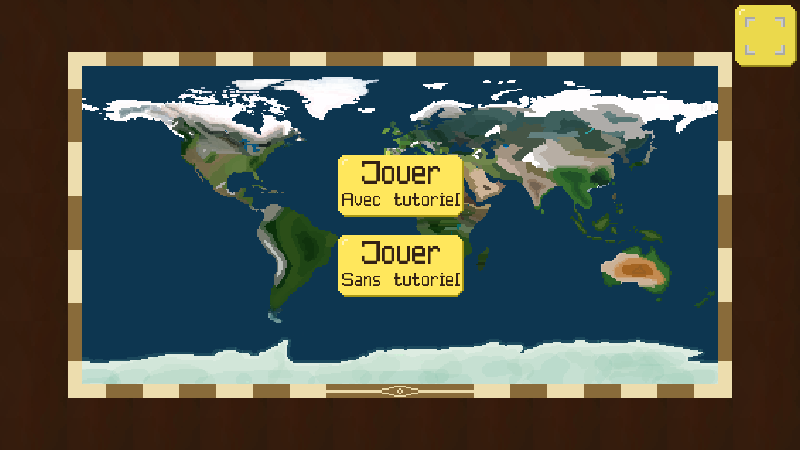
\includegraphics[width=\linewidth]{../images/mainMenu}
                \caption{Menu principal du jeu}
                \label{fig:mainMenu}
        \end{figure}

        Figure \ref{fig:mainMenu}

        \href{https://www.latex-tutorial.com/tutorials/pgfplots/}{Lien vers le tuto}



\end{document}
